\RequirePackage{cmap}

\documentclass[conference]{IEEEtran}[2015/08/26]
\usepackage[T1]{fontenc}
\usepackage[utf8]{inputenc}
\usepackage[indonesian]{babel}
\usepackage{mwe}
\usepackage[zerostyle=b,scaled=.75]{newtxtt}
\usepackage{booktabs}
\usepackage{graphicx}

\usepackage{listings}
\lstset{
  basicstyle=\ttfamily,
  columns=fixed,
  basewidth=.5em,
  xleftmargin=0.5cm,
  captionpos=b
}

\usepackage{upquote}
\usepackage{balance}
\usepackage[square,comma,numbers,sort&compress]{natbib}

\renewcommand{\bibfont}{\normalfont\footnotesize}

\usepackage{etoolbox}
\makeatletter
\patchcmd{\NAT@test}{\else \NAT@nm}{\else \NAT@hyper@{\NAT@nm}}{}{}
\makeatother

\usepackage{hyperref}

\hypersetup{hidelinks,
  colorlinks=true,
  allcolors=black,
  pdfstartview=Fit,
  breaklinks=true
}

\usepackage[all]{hypcap}

\usepackage[caption=false,font=footnotesize]{subfig}

\usepackage{stfloats}

\hyphenation{
}

\begin{document}

  % Ubah kalimat berikut sesuai dengan judul penelitian.
\title{Kalkulasi Energi pada Roket Luar Angkasa \\ Berbasis \emph{Anti-Gravitasi}}

% Ubah kalimat-kalimat berikut sesuai dengan nama, institusi, alamat dan kontak penulis.
\author{
  \IEEEauthorblockN{Elon Reeve Musk}
  \IEEEauthorblockA{Departemen Teknik Dirgantara\\
    Fakultas Teknologi Dirgantara\\
    Institut Teknologi Sepuluh Nopember\\
    Surabaya, Indonesia 60111\\
    elon.musk@mhs.its.ac.id}

  \and
  \IEEEauthorblockN{Nikola Tesla}
  \IEEEauthorblockA{Departemen Teknik Dirgantara\\
    Fakultas Teknologi Dirgantara\\
    Institut Teknologi Sepuluh Nopember\\
    Surabaya, Indonesia 60111\\
    \url{https://nikolatesla.me}}

  \and
  \IEEEauthorblockN{Wernher von Braun}
  \IEEEauthorblockA{Departemen Teknik Dirgantara\\
    Fakultas Teknologi Dirgantara\\
    Institut Teknologi Sepuluh Nopember\\
    Surabaya, Indonesia 60111\\
    von.braun@td.its.ac.id}
}

% Digunakan untuk menampilkan judul dan deskripsi penulis.
\maketitle

  % Mengubah keterangan `Abstract` ke bahasa indonesia.
% Hapus bagian ini untuk mengembalikan ke format awal.
\renewcommand\abstractname{Abstrak}

\begin{abstract}

  % Ubah paragraf berikut sesuai dengan abstrak dari penelitian.
  Pada penelitian ini kami mengajukan \lipsum[1][1-12]

\end{abstract}

% Mengubah keterangan `Index terms` ke bahasa indonesia.
% Hapus bagian ini untuk mengembalikan ke format awal.
\renewcommand\IEEEkeywordsname{Kata kunci}

\begin{IEEEkeywords}

  % Ubah kata-kata berikut sesuai dengan kata kunci dari penelitian.
  Roket, Anti-gravitasi, Energi, Angkasa.

\end{IEEEkeywords}


  \section{Pendahuluan}
\label{sec:pendahuluan}

Selama beberapa tahun terakhir, robot telah mengalami perkembangan yang signifikan dari robot beroda untuk edukasi \citep{goncalves2009} hingga robot manipulator untuk skala industri \citep{Blatnicky2020}.
Salah satu bentuk perkembangan lain dari robot tersebut adalah \emph{socially assistive robots} (SARs).
SARs merupakan jenis robot dalam bidang \emph{socially assistive robotics} yang menggabungkan aspek yang ada pada \emph{assistive robotics} dan \emph{socially interactive robotics} sehingga menjadikan SARs sebagai robot yang mampu memberikan bantuan kepada pengguna dalam bentuk interaksi sosial \citep{seifer2005}.

Namun, karena sifat dari SARs yang melibatkan interaksi langsung dengan pengguna, maka pengujian dari robot akan menjadi sulit dan beresiko bagi pengguna yang ikut terlibat dalam pengujian tersebut \citep{erickson2020}.
Salah satu solusi untuk mengatasi masalah tersebut adalah dengan melakukan pengujian secara virtual melalui simulasi robot.
Selain bisa meminimalisir resiko, penggunaan simulasi robot sebagai media pengujian robot juga bisa mengurangi biaya yang dibutuhkan dan menghemat waktu pengujian selama pengembangan robot tersebut \citep{takaya2016}.

Hingga saat ini sudah ada beberapa simulator yang bisa digunakan untuk menjalankan simulasi robot seperti Webots \citep{michel2004}, Gazebo \citep{koenig2004}, V-REP \citep{rohmer2013}, OpenAI Gym \citep{brockman2016}, dan lain sebagainya.
Namun, simulator-simulator tersebut hanyalah platform yang secara umum digunakan untuk membantu pengembangan robot melalui simulasi virtual.
Sedangkan pengembangan dari lingkungan simulasi dan kontroler robot untuk simulasi tersebut harus dibuat sendiri oleh pengembang robot.

Untuk itu, pada penelitian ini kami mengajukan penelitian terkait pengembangan lingkungan simulasi untuk pengujian SARs menggunakan ROS 2 dan Gazebo.
ROS 2 dan Gazebo sendiri dipilih karena tersedianya banyak library yang dapat membantu pengembangan maupun pengujian robot, terutama untuk simulasi.
Selain itu, dengan adanya ROS 2, kontroler robot yang diuji melalui simulasi bisa dengan mudah dipindahkan ke robot fisik untuk diuji secara langsung pada pengguna \citep{takaya2016}.

  \section{Penelitian Terkait}
\label{sec:penelitianterkait}

Beberapa penelitian sebelumnya telah berhasil dalam mengembangkan lingkungan simulasi untuk robot menggunakan ROS (Pendahulu ROS 2) dan Gazebo.
Seperti yang dilakukan Qian et al. \citep{qian2014} yang mengembangkan simulasi untuk robot \emph{manipulator}, Zhang et al. \citep{zhang2015} yang mengembangkan simulasi untuk robot \emph{quadrotor UAV}, dan Takaya et al. \citep{takaya2016} yang mengembangkan lingkungan simulasi untuk pengujian terhadap \emph{mobile robot}.
Namun, berbeda dengan penelitian yang telah dilakukan sebelumnya, penelitian yang akan kami lakukan memilih menggunakan ROS 2 agar kontroler robot yang dibuat untuk simulasi memiliki performa yang lebih baik serta dapat bekerja secara \emph{real-time} \citep{maruyama2016}.

Selain itu, penelitian lain juga telah dilakukan oleh Erickson et al. \citep{erickson2020} yang mengembangkan Assistive Gym, sebuah \emph{framework} simulasi untuk \emph{assistive robotics} berbasis OpenAI Gym.
\emph{Framework} simulasi tersebut kemudian digunakan oleh Clegg et al. \citep{clegg2020} untuk mengembangkan metode \emph{learning} melalui simulasi pada kolaborasi antara robot dengan manusia dalam membantu pemakaian baju pada manusia.
Namun, karena tidak menggunakan ROS, kontroler robot yang dibuat untuk simulasi yang menggunakan \emph{framework} tersebut perlu dibuat ulang ketika akan diujikan secara langsung pada pengguna menggunakan robot fisik.
Walaupun begitu, penelitian yang dilakukan oleh Zamora et al. \citep{zamora2016} menunjukkan bahwa simulasi yang ada pada OpenAI Gym juga bisa diintegrasikan pada ROS dan Gazebo, sehingga tidak menutup kemungkinan bahwa Assistive Gym juga bisa digunakan bersamaan dengan ROS 2 dan Gazebo.

  \section{ROS 2 dan Gazebo}
\label{sec:rosgazebo}

\subimport{3-ros-gazebo}{a-ros2.tex}
\subimport{3-ros-gazebo}{b-gazebo.tex}

  \section{Desain Sistem}
\label{sec:desainsistem}

\subsection{Desain Robot yang Digunakan}
\label{subsec:desainrobot}

\begin{figure} [ht]
  \centering
  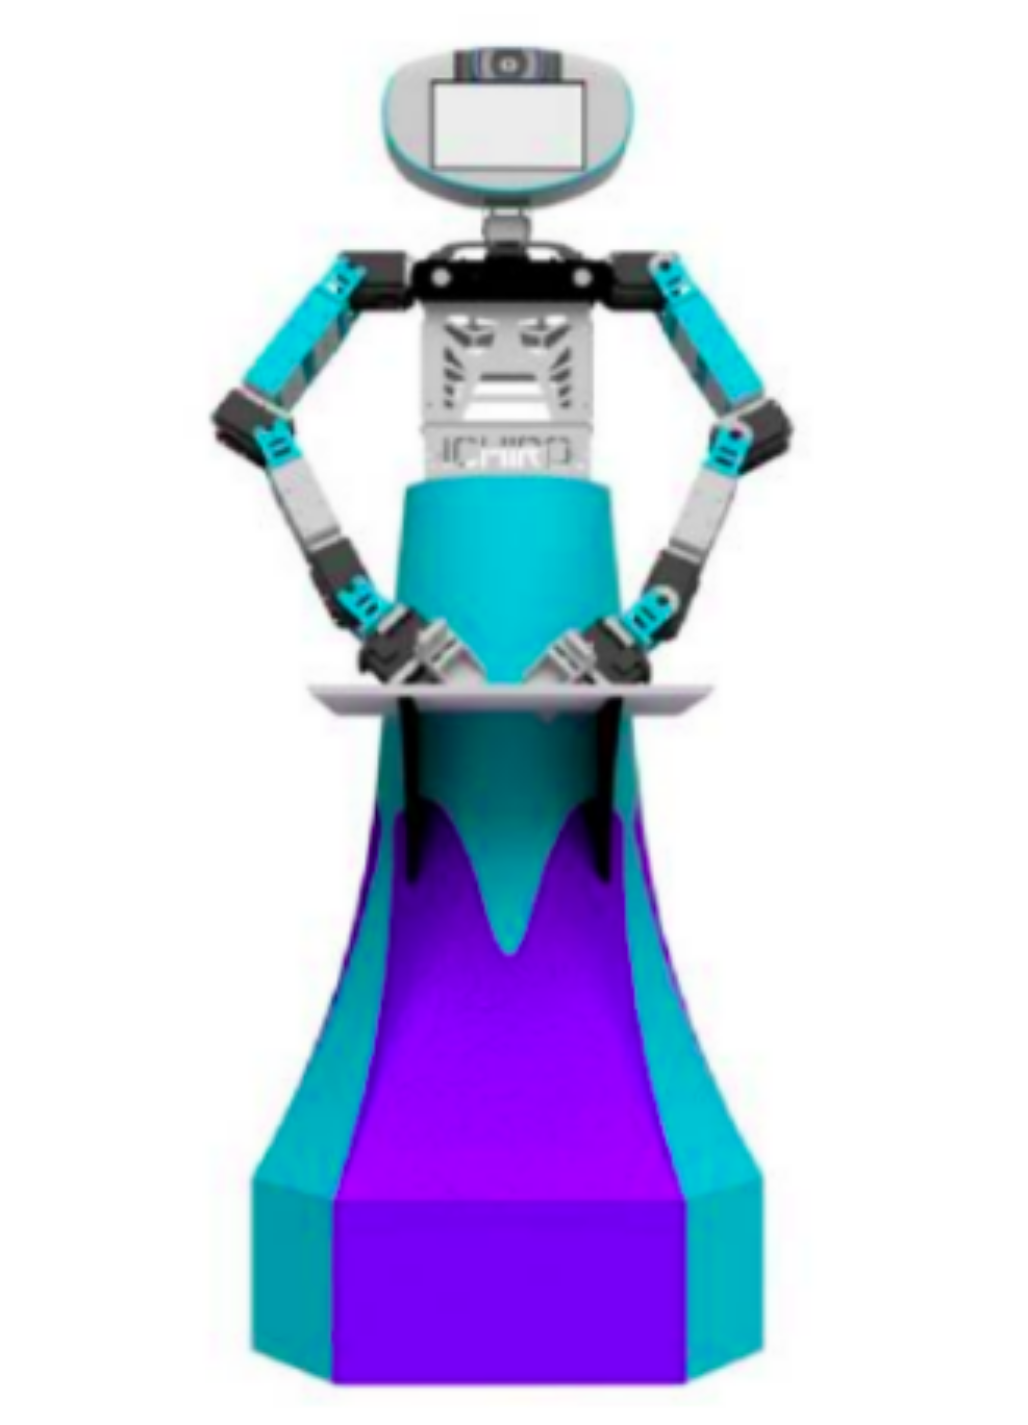
\includegraphics[scale=0.55]{gambar/desainrobot.png}
  \caption{Diagram desain robot \emph{Dienen}.}
  \label{fig:desainrobot}
\end{figure}

Robot yang akan digunakan pada pada penelitian ini adalah robot \emph{Dienen} yang merupakan kelanjutan dari robot \emph{IRIS} \citep{dikairono2020}\citep{zanuar2019} dengan penambahan desain dari robot \emph{ICHIRO} \citep{muhtadin2019} di bagian atas robot.
Desain seperti ini secara umum dikenal sebagai desain \emph{mobile humanoid robot} \citep{mohamed2012}, yang merupakan desain gabungan antara robot \emph{mobile} dan robot \emph{humanoid}.
Seperti yang terlihat pada Gambar \ref{fig:desainrobot}, bagian bawah robot menyerupai robot \emph{mobile} dengan penggerak \emph{omnidirectional wheels} yang memungkinkan pergerakan robot secara \emph{holonomic} ke segala arah\citep{oliveira2008}, sedangkan bagian atas robot menyerupai robot \emph{humanoid} yang terdiri atas badan, kepala, dan lengan.
Dengan desain \emph{mobile humanoid robot} ini, diharapkan pengguna bisa merasakan interaksi sosial yang lebih baik dengan robot karena memiliki bentuk mendekati manusia \citep{rossi2018} sekaligus mempermudah navigasi dari robot ke berbagai tempat.

Robot \emph{Dienen} dilengkapi dengan beberapa sensor seperti IMU (\emph{inertial measurement unit}) untuk mengetahui orientasi dari robot, \emph{rotary encoder} untuk melakukan perhitungan odometri dari robot, \emph{distance sensor} untuk mendeteksi adanya objek lain di sekitar robot, sensor kamera di kepala untuk menangkap citra, dan sensor \emph{depth camera} yang nantinya bisa digunakan untuk melakukan pemetaan dari ruangan.
Selain itu robot ini juga dilengkapi dengan dua lengan seperti robot \emph{manipulator} yang bisa diatur pada berbagai posisi dan orientasi \citep{iqbal2012}.
Dengan adanya sensor dan aktuator ini diharapkan robot mampu melakukan tindakan \emph{assistive} secara sosial sesuai dengan data yang didapatkan dari sensor yang ada.

\subsection{Desain Kontroler Robot}
\label{subsec:desainkontroler}

\begin{figure} [ht]
  \centering
  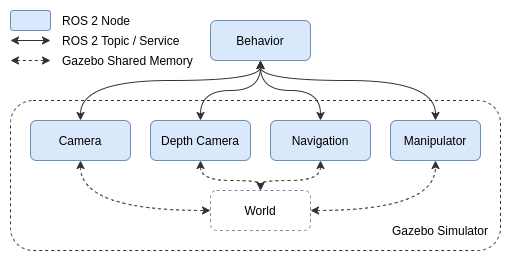
\includegraphics[scale=0.45]{gambar/kontrolersimulasi.png}
  \caption{Diagram sistem kontroler robot di simulasi.}
  \label{fig:kontrolersimulasi}
\end{figure}

Kontroler robot yang digunakan untuk simulasi ini akan dikembangkan menggunakan ROS 2.
Kontroler tersebut akan dipisah menjadi beberapa bagian dalam bentuk \emph{ROS 2 node} seperti yang terlihat pada Gambar \ref{fig:kontrolersimulasi}.
Setiap \emph{node} yang ada akan terhubung satu sama lain menggunakan sistem komunikasi antar proses ROS 2 yang berupa \emph{topics} dan \emph{services}.

Bagian utama dari kontroler robot tersebut adalah \emph{node behavior} yang berisi program yang mengatur segala tindakan robot berdasarkan data yang didapat dari sensor yang ada di simulasi.
Kemudian \emph{node Behavior} tersebut akan terhubung dengan empat \emph{node} lain yang merepresentasikan sensor dan aktuator yang ada pada robot.
Keempat \emph{node} tersebut akan terpasang di dalam cakupan simulator Gazebo sebagai \emph{Gazebo plugins}, sehingga mampu digunakan untuk mengakses dan memanipulasi data yang ada di simulasi menggunakan sistem \emph{shared memory} pada Gazebo \citep{gazeboplugins}.

\begin{figure} [ht] \centering
  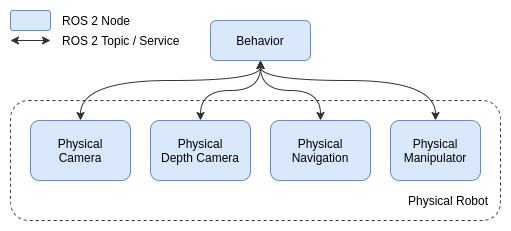
\includegraphics[scale=0.45]{gambar/kontrolerfisik.png}
  \caption{Diagram sistem kontroler robot untuk robot fisik.}
  \label{fig:kontrolerfisik}
\end{figure}

Sistem ini dirancang secara terpisah agar \emph{node Behavior} yang diujikan di lingkungan simulasi bisa langsung bekerja pada robot fisik.
Seperti yang terlihat pada Gambar \ref{fig:kontrolerfisik}, transfer kontroler ke robot fisik dapat dilakukan dengan mengubah keseluruhan cakupan yang ada di simulator Gazebo, yang berupa empat \emph{node} yang telah disebutkan sebelumnya, menjadi \emph{node} yang memproses sensor dan aktuator yang ada pada robot fisik.
Dengan ini pengujian yang dilakukan di simulasi bisa langsung diterapkan ketika diujikan pada robot fisik karena tidak perlunya pembuatan ulang kontroler yang menyesuaikan sistem yang ada pada robot.


  \section{Evaluasi}
\label{sec:evaluasi}

\lipsum[1-5]

  \section{Kesimpulan}
\label{sec:kesimpulan}

\lipsum[6-8]


  \bibliographystyle{IEEEtranN}
  \bibliography{pustaka/pustaka.bib}

  \balance

\end{document}
